\section{Spyware Abuse of Android APIs}
\label{sec:api-abuse}

In this section, we explain how spyware apps implement various privacy invasive
capabilities using existing APIs supported by the Android OS.
%These different capabilities enable attackers to achieve various goals: monitor a user's online activities (e.g., the messages they send, the photos they take, etc.), abuse the device to spy on the user's activity in the physical world (e.g., using the victim's phone to silently record audio and video or track their location), stealthily spy on their victim without their knowledge or consent, and persistently conduct their spying over a long period of time.
We start by discussing our methodology for identifying these capabilities and uncovering their associated implementations.
We then summarize the set of basic capabilities (\S~\ref{subsec:features_enabled_by_permission}) that either do not require any permissions or are enabled just by acquiring permissions,
and group
all of the other capabilities that we study into three categories based on their goals: stealthily
collecting a victim's information (\S~\ref{subsec:data_gathering}), hiding the app's presence on the phone (\S~\ref{subsec:hiding_the_app}), and persistently
spying over a long period of time (\S~\ref{subsec:persistence}).
For each category, we
describe
each capability in the category and its associated implementations, and end
the category by discussing potential mitigations.
%We conclude this section with a short discussion.

%\grant{Suggestion for an extra overview sentence: These different features
%enable attackers to achieve four invasive goals: monitor a user's online
%activities (e.g., the messages they send, the photos they take, etc.), abuse the
%device to spy on the user's activity in the physical world (e.g., using the
%victim's phone to silently record audio and video or track their location),
%stealthily spy on their victim without their knowledge or consent, and
%persistently conduct their spying over a long period of time.} \grant{My
%suggested wording above is a bit clunky, but I think it would be helpful to
%structure these features in terms of slightly high-level goals that stalkers
%want to achieve (capturing different kinds of the victim's digital + physical
%activity, stealthily performing their spying, and being able to spy on the
%victim for long periods of time) and present an overview of this framing
%upfront.}

%We start by describing how we select the features and our methodology for
%uncovering implementations associated with each feature
%(Section~\ref{subsec:misuse_discovery}). Next, we present X features and their
%implementations, and discuss potential mitigation solutions
%(Section~\ref{subsec:api_abuse_results}).

% \begin{figure*}[h]
% \includegraphics[width=\textwidth]{fig/APIAbuse.pdf}
% \caption{Summary of features studied}
% \label{tab:feature_summary}
% \end{figure*}



\begin{table*}[h]
  \centering
    \begin{tabular}{p{3.0cm}p{4.7cm}llllllllllllll}
       Category                                                &Capabilities                          &\rotatebox{90}{mSPY}  &\rotatebox{90}{Mobile-tracker-free}  &\rotatebox{90}{Clevguard}  &\rotatebox{90}{HoverWatch}  &\rotatebox{90}{Flexispy}  &\rotatebox{90}{Spyic}  &\rotatebox{90}{Spyhuman}  &\rotatebox{90}{TheTruthSpy}  &\rotatebox{90}{iKeyMonitor}  &\rotatebox{90}{Cerberus}  &\rotatebox{90}{Spy24}  &\rotatebox{90}{Spapp}  &\rotatebox{90}{Meuspy}  &\rotatebox{90}{Highstermobile}  \\
      \midrule
    \multirow{11}{*}{\shortstack[l]{Basic Capabilities (\S~\ref{subsec:features_enabled_by_permission})}}   &Ambient Recording                     &                      &\checkmark                           &                 &                            &\checkmark                &                       &\checkmark                &\checkmark                   &\checkmark                   &\checkmark                &\checkmark             &\checkmark             &\checkmark              &                                \\
                                                                                                     &Calendar                              &\checkmark            &\checkmark                           &\checkmark                 &\checkmark                  &\checkmark                &\checkmark             &\checkmark                &\checkmark                   &\checkmark                   &\checkmark                &\checkmark             &\checkmark             &\checkmark              &\checkmark                      \\
                                                                                                     &Call Logs                             &\checkmark            &\checkmark                           &\checkmark                 &\checkmark                  &\checkmark                &\checkmark             &\checkmark                &\checkmark                   &\checkmark                   &\checkmark                &\checkmark             &\checkmark             &\checkmark              &\checkmark                      \\
                                                                                                     &Clipboard                             &                      &\checkmark                           &                           &                            &                          &                       &                          &\checkmark                   &\checkmark                   &                          &\checkmark             &                       &                        &                                \\
                                                                                                     &Contacts                              &\checkmark            &\checkmark                           &\checkmark                 &\checkmark                  &\checkmark                &\checkmark             &\checkmark                &\checkmark                   &\checkmark                   &\checkmark                &\checkmark             &\checkmark             &\checkmark              &\checkmark                      \\
                                                                                                     &Info of Other Applications            &\checkmark            &\checkmark                           &\checkmark                 &\checkmark                  &\checkmark                &\checkmark             &\checkmark                &\checkmark                   &\checkmark                   &\checkmark                &\checkmark             &\checkmark             &\checkmark              &\checkmark                      \\
                                                                                                     &Location                              &\checkmark            &\checkmark                           &\checkmark                 &\checkmark                  &\checkmark                &\checkmark             &\checkmark                &\checkmark                   &\checkmark                   &\checkmark                &\checkmark             &\checkmark             &\checkmark              &\checkmark                      \\
                                                                                                     &Network Info                          &\checkmark            &\checkmark                           &\checkmark                 &\checkmark                  &\checkmark                &\checkmark             &\checkmark                &\checkmark                   &\checkmark                   &\checkmark                &\checkmark             &\checkmark             &\checkmark              &\checkmark                      \\
                                                                                                     &Phone Info                            &\checkmark            &\checkmark                           &\checkmark                 &\checkmark                  &\checkmark                &\checkmark             &\checkmark                &\checkmark                   &\checkmark                   &\checkmark                &\checkmark             &\checkmark             &\checkmark              &\checkmark                      \\
                                                                                                     &SMS or MMS                            &\checkmark            &\checkmark                           &\checkmark                 &\checkmark                  &\checkmark                &\checkmark             &\checkmark                &\checkmark                   &\checkmark                   &\checkmark                &\checkmark             &\checkmark             &\checkmark              &\checkmark                      \\
                                                                                                     &Shared Media Files                    &\checkmark            &\checkmark                           &\checkmark                 &\checkmark                  &\checkmark                &\checkmark             &\checkmark                &\checkmark                   &\checkmark                   &\checkmark                &\checkmark             &\checkmark             &\checkmark              &\checkmark                      \\
    \hline
%    \multirow{4}{*}{\shortstack[l]{\S~3.3}} & \multirow{4}{*}{\shortstack[l]{Data Gathering}}         &Invisible camera access               &                      &\checkmark                           &\checkmark                 &\checkmark                  &\checkmark                &                       &\checkmark                &\checkmark                   &\checkmark                   &\checkmark                &\checkmark             &\checkmark             &\checkmark              &\checkmark                      \\
    \multirow{4}{*}{\shortstack[l]{Data Gathering (\S~\ref{subsec:data_gathering})}}         &Invisible camera access               &                      &\checkmark                           &\checkmark                 &\checkmark                  &\checkmark                &                       &\checkmark                &\checkmark                   &\checkmark                   &\checkmark                &\checkmark             &\checkmark             &\checkmark              &\checkmark                      \\
                                                                                                     &Invisible microphone access                  &                      &\checkmark                           &\checkmark                 &\checkmark                  &\checkmark                &                       &\checkmark                &\checkmark                   &\checkmark                   &                          &\checkmark             &\checkmark             &\checkmark              &                                \\
                                                                                                     &Accessing protected data               &\checkmark            &\checkmark                           &\checkmark                 &\checkmark                  &\checkmark                &\checkmark             &\checkmark                &\checkmark                   &\checkmark                   &\checkmark                &\checkmark             &\checkmark             &\checkmark              &\checkmark                      \\
                                                                                                     &Taking screenshots                    &\checkmark            &\checkmark                           &\checkmark                 &\checkmark                  &                          &                       &\checkmark                &                             &\checkmark                   &                          &\checkmark             &\checkmark             &\checkmark              &                                \\
    \hline
%    \multirow{3}{*}{\shortstack[l]{\S~3.4}} & \multirow{3}{*}{\shortstack[l]{Hiding the App}}  &Hiding app icon                       &\checkmark            &\checkmark                           &\checkmark                 &\checkmark                  &\checkmark                &\checkmark             &\checkmark                &\checkmark                   &\checkmark                   &\checkmark                &\checkmark             &\checkmark             &\checkmark              &                                \\
    \multirow{3}{*}{\shortstack[l]{Hiding the App (\S~\ref{subsec:hiding_the_app})}}  &Hiding app icon                       &\checkmark            &\checkmark                           &\checkmark                 &\checkmark                  &\checkmark                &\checkmark             &\checkmark                &\checkmark                   &\checkmark                   &\checkmark                &\checkmark             &\checkmark             &\checkmark              &                                \\
                                                                                                     &Launching a hidden app                &                      &\checkmark                           &                           &\checkmark                  &\checkmark                &\checkmark             &\checkmark                &\checkmark                   &\checkmark                   &\checkmark                &\checkmark             &\checkmark             &\checkmark              &                                \\
                                                                                                     &Hide from recents screen              &\checkmark            &\checkmark                           &\checkmark                 &\checkmark                  &\checkmark                &\checkmark             &\checkmark                &                             &\checkmark                   &\checkmark                &\checkmark             &                       &\checkmark              &\checkmark                      \\
    \hline
%    \multirow{2}{*}{\shortstack[l]{\S~3.5}} & \multirow{2}{*}{\shortstack[l]{Persistence}}            &Obscuring the uninstallation process  &\checkmark            &\checkmark                           &\checkmark                 &                            &\checkmark                &                       &\checkmark                &\checkmark                   &\checkmark                   &\checkmark                &\checkmark             &\checkmark             &\checkmark              &                                \\
    \multirow{2}{*}{\shortstack[l]{Persistence (\S~\ref{subsec:persistence})}}            &Obscuring the uninstallation process  &\checkmark            &\checkmark                           &\checkmark                 &                            &\checkmark                &                       &\checkmark                &\checkmark                   &\checkmark                   &\checkmark                &\checkmark             &\checkmark             &\checkmark              &                                \\
                                                                                                     &Creating "diehard" services           &\checkmark            &\checkmark                           &\checkmark                 &\checkmark                  &\checkmark                &\checkmark             &\checkmark                &\checkmark                   &\checkmark                   &\checkmark                &\checkmark             &\checkmark             &\checkmark              &\checkmark                      \\
    \hline
    \end{tabular}
    \caption{Summary of capabilities studied. A star denotes that an app implements a particular capability.
      %, otherwise we leave the corresponding cell in the table blank.
      \label{tab:feature_summary}}
  \end{table*}



\subsection{Methodology}
\label{subsec:misuse_discovery}


%% \geoff{I'm now thinking that we can use Section 2 to set the context:
%%   how spyware is used + our app selection process.  we'll then put the
%%   methodologies back into Sections 3 and 4.}

% Breaking into the vault: Privacy, security and forensic analysis of Android vault applications
% Transfiguring of an Android App Using Reverse Engineering
% Reverse engineering of mobile applications
% https://www.uit.edu.mm/storage/2020/09/No.-5.pdf
We gather a list of privacy invasive capabilities from two sources: (1)
capabilities advertised and offered by spyware apps; and (2) prior
academic papers and industry reports described in Section~\ref{sec:related_work} that look at how the Android API
can be used to achieve such unintended functionality.
Table~\ref{tab:feature_summary} summarizes the capabilities we study
and shows which spyware apps implement them.
To understand how the spyware apps implement their nefarious capabilities, we reverse engineered and analyzed each app. Our approach consists of three steps.

\textbf{Preparation.} We acquire the latest APKs of spyware apps by directly downloading them from their websites. We use \texttt{APKTOOL}~\cite{ApktoolA72:online} to disassemble the APKs and obtain the corresponding manifest and smali code.\footnote{Smali is a human-readable represenation of the Dalvik bytecode used by Android apps.} We also decompile the APK to Java source using \texttt{JADX}~\cite{skylotja9:online}. Identifiers and even strings in the Java code are often obfuscated, and Appendix~\ref{sec:apk_obfuscation} provides more details about the obfuscation used
by various apps.

\textbf{Manual Investigation.}
For each capability, we manually analyzed the app manifest and the decompiled Java code to determine how
each capability was implemented using the standard Android API: we manually located the API primitives associated with each capability, examined the relevant control flow, and confirmed that the primitives we identified were reachable. While we primarily used the decompiled Java code for
analysis, we reviewed the smali code when necessary (e.g., when a function fails
to decompile). Since the variable and method names were often obfuscated, we renamed them to human-readable ones as we examined the decompiled Java code (our naming annotations are available upon request).

Once we discovered an implementation for a particular capability and
the API primitives one app used, we expedited our search process
for other apps by searching for use of the same API primitives, and manually
reviewed the results to remove false positives. If this API similarity
approach did not yield results, we reverted back to manually
inspecting the code.

We use two heuristics to guide our manual investigation process.
First, many apps can receive remote commands (e.g., using third-party
libraries such as Firebase~\cite{Firebase21:online}).  The method
responsible for dispatching remote commands is a useful top-down
starting place for identifying the underlying implementation (e.g.,
following the methods it calls in response to remote commands).  For
apps that do not receive remote commands, they operate as background
services to covertly collect user data. These background services
often are responsible for dispatching various tasks and contain useful
leads. Second, for any capability, there are limited ways to implement
it using Android API primitives, and many of them are publicly
documented (e.g., capturing audio through \texttt{MediaRecorder}). Searching for these API primitives in the code helps to
quickly locate methods associated with a capability. Additionally,
once we identified an implementation of a capability, we examined its
control flow in a bottom-up fashion to identify the operation that
would trigger its execution (typically leading back to dispatch
methods).

\textbf{Confirmation.} For each implementation of a capability (and
related API primitives) we discover, we verified our analysis conclusions
by developing an app using the same API primitives and
testing it on a Pixel 4 phone running Android 11. We also installed and ran each spyware app to ensure the capabilities we observed were indeed enabled.
Since the majority of the apps we
study have been implemented using Android APIs up to Android 11, we
discuss their implementations in that context. However, we also
discuss the impact changes in Android 12 can have on the spyware apps.

%\subsubsection{Code Release}
\textbf{Code Release.}  Our code that implements all the API
primitives discovered in this paper is available upon
request. Similarly, the annotated class and variable names are
available upon request (which can be used to reproduce our results
after independently acquiring the corresponding APK files). To avoid
potential copyright infringement risks, we do not provide the
decompiled and annotated source code itself.

%% We focus our discussion on Android 11 and earlier, and discuss the
%% impact of Android 12 when relevant. \alex{We need a machine that runs
%%   Android 12? Big enhancements include a persistent indicator and
%%   privacy dashboard}


%\subsection{Abusive and Non-abusive API Usage}
%\alex{maybe this is not necessary}
%We define Android API misuse as: any functionality that relies on using the
%Android platform API in ways that violate either Play Store policies or the
%clearly intended usage of the platform per the Android developer documentation.
%Broadly speaking, we focus on abusing API to: covertly collect private user or
%app data, hide app traces, and survive across reboots and kills.


% \subsection{Results}
% \label{subsec:api_abuse_results}
% We start by briefly discussing a set of features that are enabled after
% acquiring certain permissions. These features are only protected by
% permissions and many are not noticeable by users. Next, we detail how spyware
% apps implement features that allow them to exfiltrate data covertly, stay
% stealthy, and persist on the target device.

\subsection{Basic Capabilities}
\label{subsec:features_enabled_by_permission}
As seen in Table~\ref{tab:feature_summary}, all spyware apps support a large, common set of basic capabilities for collecting sensitive user data.
These capabilities either do not require any permission (e.g., clipboard) or are easily enabled after obtaining particular Android permissions (e.g., reading SMS messages, contacts, call logs, etc.). Spyware apps can obtain these capabilities simply by
requesting the associated permissions in the manifest at installation or their first run.
Additionally, by design most of these capabilities
(except for location and ambient recording) do not provide any notification to
the user and are straightforward to implement.


\subsection{Data Gathering}
\label{subsec:data_gathering}
Spyware apps seek to stealthily collect a victim's information without being noticed. In this section, we describe how they covertly access the camera, the microphone, and protected data of other apps, as well as how they take screenshots all without the victim's knowledge.

\subsubsection*{Capability \#1: Invisible Camera Access}
\label{subsubsec:invisible_cam}
Spyware apps use a device's camera to take pictures, record videos, and stream live
videos. To remain hidden from the victim, spyware apps need to access the camera
without being noticed. The apps we studied use three methods to achieve
surreptitious camera access: (1) using an invisible preview; (2) intercepting raw
frames without a preview; and (3) using an invisible browser.
% \alex{added a novelty statement}
While the first technique is well-documented in the malware literature (e.g., Yan et al.~\cite{yan2019understanding}), the second and third techniques
have not been reported before and reflect
the creativity that spyware authors continue to apply in
abusing the Android API to implement their capabilities.

% (unique to Spy24);

% We start by briefly explaining how camera works. Readers who are interested in
% the details should refer to Android's developer
% guide~\cite{Cameraca74:online}. Android apps can capture images or videos by
% creating a camera capture session. To create a camera session, apps need to
% provide it with one or more output target buffers. One type of target buffer
% is SurfaceView, which can be used as a preview to display the image or video
% directly to the user. Other types of target buffers include ImageReader and
% SurfaceTexture, which are used for more advanced scenarios and not visible to
% users. If spyware apps uses SurfaceView as the target buffer, they need to
% hide the preview being displayed. This can be done by setting the preview size
% to 1x1.

% they can stay unnoticed by creating a SurfaceView that is not visible
% (typically of size 1x1).

\textbf{Invisible Preview}. One way to use the camera is to create a preview that displays an image or video to users. Once a preview is started, apps can take pictures or record videos. Benign apps (such as selfie apps) use a preview so that users can see the current status of the camera. Spyware apps, in contrast, seek to hide this preview by setting the preview to an invisible size (typically a 1x1 pixel) or making the preview transparent.
% \alex{moved the novelty statement up}

\textbf{Raw Frames Without a Preview}.
Spyware apps can also access the output of the camera without displaying a
preview using advanced camera features supported by
Android~\cite{Cameraca74:online}. For example, apps can capture raw frames from
the camera with either an \texttt{ImageReade}r~\cite{Cameraca74:online} or
\texttt{SurfaceTexture}~\cite{SurfaceT78:online}, neither of which requires showing a
preview on the screen.
Benign apps (such as photo apps) use these
features for advanced operations such as frame-by-frame processing. Spyware
apps, on the other hand, use these features to capture raw frames, either saving
the frames locally or streaming the frames to a remote server, all without the
victim noticing. While the expectation for such advanced features is that the
processed frames will be displayed to users eventually (which is normally the
case for benign apps), this by no means is enforced. Finally, we note that four
apps rely on the third-party library WebRTC (or its variants) to achieve this functionality (WebRTC uses both \texttt{ImageReader} and \texttt{SurfaceTexture}).

%\geoff{does webrtc then use an ImageReader or SurfaceTexture?}\alex{fixed}

\textbf{Invisible Browser}. Unique to Spy24, this app uses an invisible
\texttt{WebView}~\cite{WebViewA25:online} (an in-app browser) with a 1x1 pixel size for
streaming live videos. While the browser may be invisible, the app can stream
full camera resolution to a Spy24 server.
%\geoff{Alex confirm?}\alex{correct}
\texttt{WebView} allows users to browse web content in an app while providing advanced
configuration options to developers. Spy24, in this instance, programmatically sets
the user agent, enables JavaScript, and disables the cache. This configuration
flexibility provided by \texttt{WebView} is necessary for streaming via a web browser.
%% as standard web browsers like Chrome have limited configuration
%% flexibility.\geoff{by hard to achieve, you mean hard to achieve
%% invisibly?}\alex{fixed}

Once the browser is configured, it accesses the camera via a JavaScript version
of WebRTC (loaded dynamically) and streams live video back to a Spy24 server.
This approach evades static analysis that examines API calls in the APK file, as
the JavaScript file is loaded during runtime.
Listing~\ref{lst:invisible_browser_code} shows a snippet of code that
demonstrates how Spy24 streams video with an invisible browser. First, it adds the 1x1 \texttt{WebView} as an overlay.  It then sets a specific user
agent to act as a trigger. Upon contacting the server, the \texttt{WebView} loads a
JavaScript file that activates the camera if the \texttt{WebView} has the specified user
agent.

%\vspace{0.5cm}
%\hspace{-0.1\linewidth}
%\begin{minipage}{0.5\textwidth}
\begin{lstlisting}[basicstyle=\small\ttfamily,caption={Code snippet that demonstrates how Spy24 streams live video.},label={lst:invisible_browser_code},captionpos=b,float=t]
// xml layout for the webview
<WebView id="@+id/wv" layout_width="1dp" layout_height="1dp"/>
// Java code that configures the webview
WebView webView = findViewById(R.id.wv);
webView.getSettings().setUserAgentString("some_user_agent");
// Javascript code that activates the camera when loaded by the webview
userAgent.includes('some_user_agent'){
  camera.start()
}
\end{lstlisting}

%\end{minipage}

%through Android's \texttt{camera2} framework~\cite{androidh66:online} or the
%deprecated \texttt{camera} framework~\cite.

%by building their customized camera implementation with the
%\texttt{android.hardware.camera2} framework (referred to as \texttt{camera2})
%or {CameraAn8:online} (referred to as \texttt{camera}). Both \texttt{camera2}
%and \texttt{camera} allow apps to capture pictures and videos.

%\texttt{camera} requires that a \texttt{Preview} must be started before
%pictures or videos can be taken~\cite{CameraAn8:online}. Spyware apps (e.g.,
%Flexispy) hide their preview by creating an invisible preview of size 1x1 as an
%overlay, a technique that has been documented in prior
%literature~\cite{yan2019understanding,pan2018panoptispy}. As an example, we
%provide more details on how Flexispy achieves invisible camera access. First,
%Flexispy access camera APIs through a foreground service, as apps running in
%the background cannot access the camera since Android 9 (API level
%28)~\cite{CameraAn8:online}. Furthermore, it adds a 1x1 \texttt{preview} to the
%screen through \texttt{WindowManager} as an \texttt{APPLICATION\_OVERLAY} (or
%\texttt{SYSTEM\_OVERLAY} before Android 6), which is protected by the
%permission \texttt{SYSTEM\_ALERT\_WINDOW}~\cite{WindowMa73:online}.
%Additionally, Flexispy will try muting the shutter sound when taking pictures
%or videos). However, we note that this is not possible in some countries (e.g.,
%Japan) due to legal concerns~\cite{HowcanIt38:online}. Finally, we observe that
%Flexispy attempts a series of different ways to access the camera if preceding
%methods fail.

%While the above approach still works for \texttt{camera2}, it is possible to
%stealthily access camera without a \texttt{Preview} with \texttt{camera2}. This
%technique has not been uncovered by any of the prior literature to the best of
%our knowledge. \texttt{camera2} provides more diverse ways of accessing camera.
%Apps need to specify one or more output target buffers to receive the raw
%image. One of the target buffers is \texttt{ImageReader}, which allows the
%spyware apps to copy the raw image into an array of bytes and save them to disk
%without launching a preview.

\subsubsection*{Capability \#2: Invisible Microphone Access}
\label{subsubsec:audio_recording}
Spyware apps use the microphone to covertly record
ambient sound, phone calls,
and voice calls (calls made in third-party apps like WhatsApp).
Ambient recording is enabled after acquiring the Android permission
to record; below we focus on how apps achieve phone call recording and voice call
recording.

\textbf{Phone call recording} on Android has evolved over time.
%% Prior to Android~6,
%% apps easily achieved call recording by setting the audio source to a specific
%% API value. From Android~6 to~8, an Android NDK workaround is required to capture
%% both uplink (Transmit) and downlink (Receive) audio source of a call. Since
%% Android~9, call recording is only possible through Microphone.  \geoff{this
%% paragraph summarizes the next, so we'll want to go with one or the other
%% depending on desired level of detail}
%
Prior to Android~6, apps could easily use \texttt{MediaRecorder} to
record phone calls~\cite{MediaRec53:online}.
% \geoff{parameter to what?}\alex{to voice call?} to \texttt{VOICE\_CALL}.
Specifying \texttt{MediaRecorder.AudioSource.VOICE\_CALL},
an app can receive both uplink and downlink audio
for a call. Since Android~6, \texttt{VOICE\_CALL} is protected by a permission
reserved for system apps and cannot be requested by third-party
apps~\cite{VOICECAL55:online}. Spyware apps (and other recording apps) use
native code via the Android NDK to circumvent this limitation, specifying
\texttt{VOICE\_CALL} by calling functions defined in
\texttt{libmedia.so}~\cite{ViktorDe77:online}.
%% ~\alex{Note, we studied the cited
%%   open-source implementation on Github instead of reverse engineering the native
%% code}.
Android~9 subsequently prevented this workaround by filtering out
unauthorized attempts to set \texttt{AudioSource}~\cite{coplukAC3:online,
  services10:online}.

After Android~9, spyware apps started recording phone calls using
Microphone, which nominally only captures uplink audio.  However, spyware apps
employ several workarounds to also capture downlink audio.  For instance, some
spyware apps turn on the speaker and turn off noise-cancelling during a phone
call so that the microphone can potentially capture downlink audio via the
speaker.
%% Related resources:
%% https://www.boldbeast.com/forum/topic1877-android-10-call-recording.html
%% https://nllapps.com/apps/acr/android9.htm
%% https://issuetracker.google.com/issues/112602629

%% \geoff{what is the difference between call
%% recording and voice call recording?}\alex{fixed in the beginning of this
%%   feature. Voice calls are calls made in apps like whatsapp}

\textbf{Voice call recording} --- recording calls made in third-party apps such as WhatsApp --- became possible with
Android~10 for apps that register as an accessibility service.
% \alex{more explaination}
Prior to Android~10,
recording voice calls was not possible, as Android only allowed one app to
access input audio at a time~\cite{Sharinga60:online}.  Android~10 relaxed this
restriction, allowing two apps to access input audio concurrently if one of them
is an \texttt{AccessibilityService}.  This feature was intended to allow an
accessibility service to perform voice recognition, however spyware apps quickly
abused it.  To detect that a voice call is active or a voice message is being
played, spyware apps use side-channels such as listening for specific
notifications triggered by voice calls or looking for specific actions (e.g.,
users clicking on the OK button to start the voice call) on the screen via
the accessibility interface.

\subsubsection*{Capability \#3: Accessing Protected Data}
%\alex{This section needs a bit of help. Protected vs Private}
A core feature of spyware apps is the ability to collect data that they
are not supposed to read, which includes reading protected data of other apps (e.g.,
WhatsApp messages) and recording keystrokes to other apps. Accessing this data is normally
impossible as each app runs in its own sandbox. Spyware apps achieve these
capabilities primarily by abusing the accessibility permission which does not
require rooting, echoing prior literature~\cite{fratantonio2017cloak,
kraunelis2013malware, jang2014a11y, diao2019kindness, kalysch2018android,
huang2021a11y, naseri2019accessileaks} that investigates how accessibility can
be abused.

\textbf{Reading protected data of other apps} can be performed in two ways: through
accessibility or notification. Most academic literature has focused on
accessibility, and only a few reports~\cite{VB2019Za6:online} have examined the
use of notification. Accessibility services are expected to read what is
rendered on the screen as they are designed to help disabled and impaired users.
Spyware apps abuse this capability to read information displayed by other apps
and extract sensitive information when an app (e.g., WhatsApp) is used.

Notification, on the other hand, allows spyware apps to read sensitive
information even if the spyware app is not active. While reading from a notification has
limitations (e.g., a spyware app cannot read images), nine spyware apps abuse it.
Finally, we note that, like accessibility, both benign apps and malicious apps
make use of notifications as a side-channel for accessing information: benign
apps (an example is~\cite{ReadUnre55:online}) do so to avoid triggering the ``Read Receipt'' feature, which notifies the
sender if the recipient has read the message,
%\geoff{sorry, don't know what this is :-)}\alex{fixed}
of other apps (e.g., Signal and WhatsApp), while malicious apps do so
purely to extract information.

\textbf{Recording keystrokes} is done via accessibility. Prior
work~\cite{fratantonio2017cloak,jang2014a11y,naseri2019accessileaks} has
demonstrated how the accessibility framework in Android can be abused for
recording keystrokes.
Spyware apps simply use the \texttt{getText} method, part
of Android's accessibility framework, to track all key presses from the user in
any app.
While there are built-in mechanisms to prevent \texttt{getText} from
reading sensitive information such as credentials (e.g., by setting
the attribute
\texttt{importantForAccessibility} to false), past
work~\cite{naseri2019accessileaks} has shown that these defenses are not
widely adopted. Additionally, mitigations like setting \texttt{importantForAccessibility} to
false also reduces the usability of benign apps such as screen readers.

%\damon{We should note that this defense would break screen readers.}\alex{fixed}

\subsubsection*{Capability \#4: Taking Screenshots}
\label{subsubsec:screenshot}
Spyware apps can also extract sensitive information by taking screenshots. We
observe two ways the apps in our set take screenshots: via
\texttt{MediaProjection} and \texttt{AccessibilityService}. For MediaProjection
to work, an activity is required~\cite{androidH20:online}. This approach is
nominally a challenge for spyware apps since they generally run as services and
do not have an activity. As a result, some spyware apps create temporary
activities that are transparent and not visible to users. These invisible
activities are then removed after the screenshot is taken.  Android~10 limited
apps that can start activities to a few scenarios~\cite{Restrict50:online}
(e.g., if an app is an accessibility service or has the \texttt{SYSTEM\_ALERT\_WINDOW}
permission). Such restrictions make it harder for spyware apps to use
\texttt{MediaProjection} to take screenshots, but still leaves a loophole as spyware apps
can register as an accessibility service and request the \texttt{SYSTEM\_ALERT\_WINDOW}
permission.
%\damon{this is vague, why does it not fully solve the problem?}\alex{fixed}

However, Android~11 (and later) has made it
simple for spyware apps to take screenshots by adding the
\texttt{takeScreenshot} API to \texttt{AccessibilityService}~\cite{Accessib97:online}.
This method requires no activity and is easy for spyware apps to implement.


\subsubsection{Mitigations}
Android has used a variety of approaches to mitigate some of the issues mentioned in this section.

The first approach is to pose additional restrictions on apps that seek to access certain information. One type of restriction is to require apps to be in a certain state: Android~10 restricted access to the clipboard information
to apps that are either the default input
method editor or is the app that currently has focus~\cite{Privacyc52:online}. As a result of this
patch, none of the spyware apps were able to acquire clipboard information\footnote{We are aware of a workaround~\cite{SolvedCl34:online} that can circumvent this restriction. However, it requires extensive user interaction and is not adopted by any of the spyware apps. We also note
that iKeyMonitor
attempted to evade this restriction by trying to acquire focus with an
invisible \texttt{EditText} of size 1x1. However, this attempt appears to be
unsuccessful: both iKeyMonitor and our cloned implementation fail to
read the clipboard.}. Another type of restriction is to require apps to possess additional permissions: besides requiring the permission to record audio, Android~10 further demands an app to be an accessibility service to capture audio input during phone calls. However, we note that permission-based restrictions are unlikely to be successful, as the abuser has physical access to the device and can grant arbitrary permissions.

%reduce the scope of granted permissions. 
% For example,
 
%% \geoff{how does this evade the restriction?  assume the
%% reader does not know what an EditText is}\alex{fixed}





%Android also normally plays a shutter sound when a picture is taken. Spyware
%apps attempt to mute the shutter sound before taking the picture, which works
%in most scenarios (this is not possible in Japan due to legal
%concerns~\cite{HowcanIt38:online}). \geoff{by not possible, do you mean muting
%is disabled in Japan?} Finally, Android~12 introduces a persistent green dot
%indicator that signals to the user when an app is using the camera or
%microphone.  Its new privacy dashboard~\cite{AndroidD76:online} can also help
%mitigate the problem of covertly recording videos. To better alert users when
%an app is taking pictures (which happens quickly, making it harder for users to
%notice the indicator), Android can make the indicator appear for at least a few
%seconds regardless of the action taken.

A second approach is to provide a visible indicator to the user that cannot be
dismissed while a granted permission is being used by any app.  For example,
Android has a visible persistent indicator for location and screen recording
use, and Android~12 introduced a visible indicator for microphone and camera
use. Such an indicator confirms to the user when they expect it to be used, and
alerts the user when they do not.

This approach can also fail depending on the use case.  For example, a
persistent indicator is useful to alert users to long-lasting actions
such as recording. However, a persistent indicator is unlikely to be
helpful for sub-second operations (e.g., taking a screenshot and
taking a picture),
%% as it is unlikely that users will notice the
%% indicator due to the short-live nature of these operations.
and users can sometimes miss these indicators (e.g., if the phone is
in a pocket or purse).  Moreover, benign use cases will also trigger
persistent indicators, which can then mask simultaneous spyware activity.  For example, the indicator for the microphone will be
displayed when a call is ongoing regardless of whether a spyware app
is performing call recording in the background or not.  In this case,
spyware apps can safely record calls in the background, as the
indicator is always on.  Indeed, sophisticated spyware can reduce
suspicion by carefully timing their actions (e.g., only performing an
action when the associated indicator is already triggered by another
app).

A third approach is to provide a convenient way for users to review the
permissions that have been granted to all installed apps.  Android~12 takes this
approach by introducing a privacy dashboard, which displays the
accesses in the last 24 hours to sensitive information such as location, microphone, and camera.
%% \geoff{which ... (describe the dashboard once here, no need when mentioned
%%   later)}\alex{fixed}.
While such a dashboard does require users to proactively
take action, it is a potentially useful tool for users to quickly identify
suspicious apps based upon the plethora of invasive permissions they have been
granted. We
recommend that all actions to access sensitive data should be added to the
privacy dashboard and users should be periodically notified of the existence of apps with excessive number of permissions.

Lastly, Android also employs various mechanisms that alert users of sensitive actions or potentially malicious activities. 
The most straightforward example is the deployment of Google Play Protect, which warns users when a potentially malicious app is being installed. As well, Android~9 requires a persistent notification for background apps that seek to access the camera and microphone: these apps need to run as a foreground service, which triggers a persistent notification that cannot be dismissed by the apps themselves. Finally, Android uses audio cues (e.g., a shutter sound) to notify users of operations such as audio and video recording. Sadly, we note that all these mechanisms can fail, as they can be turned off either programmatically (e.g., audio cues normally can be
turned off after acquiring permissions to manipulate audio
settings\footnote{One exception is Japan, where muting the shutter sound when
taking pictures or videos is not possible due to legal
requirements~\cite{HowcanIt38:online}.}) or by a malicious user (e.g., as mentioned in Appendix~\ref{subsubsec:install_configure}, spyware apps require that their notification be disabled by the abuser upon installation).


The research community has also proposed various defense mechanisms when
studying some of issues mentioned in this section. Huang et
al.~\cite{huang2021a11y}, for instance, seek to constrain accessibility misuse
with the assumption that the user is benign, which unfortunately does not hold
in the context of spyware apps.
%% \damon{give a succinct description of the
%%   solution in the citation.} \alex{fixed}
Another example is Petracca et
al.~\cite{petracca2015audroid}, who proposed requiring user approval before an
app can record to stop malicious apps from eavesdropping. However, we note that
this defense is unlikely to be successful as the adversary generally has physical access to the target device. On the one
hand, this defense will only work if user approval is requested every time,
which leads to significant usability issues. On the other hand, if user approval is
only requested once when an app tries to record, it is unlikely to be successful
as the abuser will have physical access to the phone and can grant the consent. Lastly, Yan et al.~\cite{yan2019understanding} developed a system for detecting overlay-based Android malware. However, their system is deployed on an Android app store and does not defend against spyware apps that are sideloaded.
%system was integrated into T-Market, an Android app store, and could not stop spyware apps from being sideloaded.

%% \geoff{the consent is only needed on install like a permission, or when an app
%% triggers recording during runtime?  sounds like the former but want to be
%% sure}\alex{fixed}

%\textbf{Mitigation.} Mitigating the issue of permissions enabling
%privacy-invasive functionality is challenging since benign apps often require
%these permissions to implement useful functionality.  The problem is made more
%challenging since a benign app (e.g., backup apps) can be abused for malicious
%purposes (e.g., data exfiltration), and there exists no reliable method to
%determine if the intention is malicious or benign~\cite{mayrhofer2021android}.
%Furthermore, abusers have physical access to the device, rendering existing
%solutions unusable.

%example is restricting access to sensitive information such as location and
%clipboard data.

%\grant{I suggest that we change the term ``data exfilitration'' to something
%like ``data capture''.  I think exfiltration will typically be interpreted as
%the process of siphoning the data off of the device and to an external source,
%but the features/capabilities below seem to be just about capturing/recording
%different data?  } This section contains a list of features supported by
%spyware apps to covertly exfiltrate data without being noticed.

%\grant{Something to consider in this section: there's a mix of different
%messages happening in this Data Exfiltration subsection: (1) we're giving an
%overview of the different kinds of data stalkerware apps can spy on, (2) we're
%highlighting that some of it can be done steathily, (3) we're talking about how
%apps get some of this data by cleverly breaking different kinds of separation
%boundaries (i.e., technical means to get functionality that they shouldn't be
%able to get).  Half of the features in this subsection seem to emphasize point
%(2) and the other half seem to emphasize point (3), which makes this data exfil
%section seem less unified on a conceptual level (e.g., is the main thing I
%should care about that that they capture X, Y, Z kinds of data? that they can
%do so stealthily? that they violate app separation mechanisms?).  I wonder if
%we could reframe the low-level wording in each feature to somehow make all of
%them about violating/bypassing user consent?  In other words, the overall
%message of this subsection is: (a) stalkerware apps want to collect information
%about users digital and physical activity (visual/audio/text/location) but (b)
%in order to collect this kind of sensitive information, an application
%typically needs to require consent either by the user (to use physical sensors
%like camera/microphone or to allow access to other applications/phone data).
%Here we analyze how attackers are able to get this data without any explicit
%consent by the users (we can still keep most of the content the same, with some
%small wording tweaks to make the stealthy spying features about bypassing
%consent for physical sensor access and the private data/screenshot features
%about bypassing consent for data/cross-app access).}

%\textbf{Mitigation.} Past literature~\cite{pan2018panoptispy,
%petracca2015audroid} has reported the potential risks of abusing the microphone
%to spy on users. Petracca et al.~\cite{petracca2015audroid} proposed requiring
%user consent before an app can record \geoff{the consent is only needed on
%install like a permission, or when an app triggers recording during runtime?
%sounds like the former but want to be sure}, which is unlikely to be successful
%in the context of IPV as the abuser will have physical access to the phone and
%can grant the consent. \geoff{we might discuss Android mitigations first (which
%exist), then what researchers have proposed}
%
%Android also has several defenses. First, Android by default plays a sound when
%a recording starts, but this audio cue can be disabled programmatically.
%Android~10 further requires that an app should be an accessibility service to
%capture audio input via the microphone~\cite{Sharinga60:online}, which spyware
%apps readily declare themselves to be.  As mentioned above, Android~12
%introduces a persistent visible indicator (green dot) that signals users when
%an app is using the camera or microphone as well as a privacy dashboard for
%reviewing permissions granted to all installed apps~\cite{AndroidD76:online}.
%While these features do not prevent spyware apps from recording calls, they do
%prevent them from doing it surreptitiously --- a significant step towards
%mitigation.

%\textbf{Mitigation.} Mitigating the abuse of accessibility or notification is
%challenging as there is no automated way to differentiate the intention of an
%app that is reading data. Huang et al.~\cite{huang2021a11y} proposes a
%framework for restricting accessibility services, but we note that this
%approach is unlikely to be successful in the context of spyware apps as they
%assume the user is benign. One potential solution is to show a persistent
%indicator for accessibility services when they are actively reading data and
%add accessibility services to the new privacy dashboard.\alex{i dont know what
%is in there} \geoff{the indicator has to be consistent with user accessibility
%(e.g., a green dot is not goin to help blind users)}

%\textbf{Mitigation.} Prior work~\cite{pan2018panoptispy} has overlooked using
%screenshots to violate privacy. The authors consider this functionality out of
%scope as Android displays a persistent indicator when the screen is being
%recorded. Due to Android's use of an indicator, most spyware apps only use
%MediaProjection to take screenshots (instead of live streaming the screen).
%Since taking a screenshot is a sub-second operation, it is unlikely that users
%will notice the indicator. Instead, we recommend that Android display the
%indicator for a few seconds regardless of the duration of the action. We also
%recommend adding the screen capture permission to the new privacy
%dashboard\alex{i dont know what is in there}.



\subsection{Hiding the App}
\label{subsec:hiding_the_app}
% This section details a list of features used by spyware apps to hide their
% activities and prevent users from discovering them.
In addition to surreptitiously spying on victims, spyware apps also use a
variety of methods to keep the existence of the app hidden from the victims.
% prevent their app from being enumerated to the user.  This section details a
% list of features used by spyware apps to hide their activities and prevent
% users from discovering them.
These tactics include hiding the app icon from the app launcher, launching a
hidden app, and hiding from the Recent screen.
%% \damon{We probably need to explain
%% some of this terminology since people might not know what the app launcher or
%% app list are conceptually. We might want to include a figure with examples of
%% these terms?} \grant{I made a slight tweak to the wording here, because I was
%% initially confused by why we have a separate stealthiness section when all of
%% the features in the previous section discuss how they steathily capture user
%% data. What this section really is about is making it so that the user cannot
%% find the app itself (rather than about having the app's functionality run
%% stealthily). The wording in my edit is not quite there yet (I'd like to make the
%% distinction more crisp, but this is minor wording/clarity stuff).}\alex{fixed}

\begin{figure}[t]
\centering
\includegraphics[width=0.95\columnwidth]{fig/app_launcher_wifi.pdf}
\caption{App launcher that displays app icons.
The Spyhuman app installed itself as the innocuous ``Wi-Fi'' icon.}
\label{fig:app_launcher}
\end{figure}

\subsubsection*{Capability \#5: Hiding App Icon}
\label{subsubsec:hide_icon}
To hide their presence,
% and make it harder for the users to noticing them,
spyware apps hide their app icons from the app launcher that lists the available
apps~\cite{whataret1:online}. Figure~\ref{fig:app_launcher} shows an example of
the app launcher, and 13 of the 14 spyware apps in our study include code to hide their
app icons from the app launcher using two methods:
% Specifically, we observe two ways to hide app icon from the app launcher:
(1) hiding the app icon at runtime, and (2) specifying no launcher activity.
% LEANBACK\_LAUNCHER~\cite{IntentAn39:online} instead of LAUNCHER.
%% \damon{again people likely do not know this terminology, such as app
%% drawer.}\alex{fixed}

\textbf{Hiding the app icon at runtime} can be implemented by invoking
the method \texttt{setComponentEnabledSetting()} and disabling the
launcher activity.  Previous work~\cite{shan2018self} examined hiding
app icons in this way, and this approach works on devices that run
Android 9 or below. An activity of category \texttt{LAUNCHER}
indicates that it should be displayed in the app
launcher~\cite{IntentAn33:online}, and disabling the launcher activity
removes the app icon from the app launcher.  Since the app is no
longer displayed in the app launcher, though, spyware apps need a
different way to launch themselves. We detail different ways to launch
apps that are not present in the app launcher in Capability \#6 below.

Since Android~10, an app's icon will appear in the app launcher even
if the launcher activity is disabled at runtime. In reaction to this
change, most spyware apps now use innocuous names and icons to
disguise the spyware app, such as ``Wi-Fi'' (as in Figure~\ref{fig:app_launcher}), ``SyncService'' and
``InternetService''.\footnote{iKeyMonitor even offers the ability to
  build apps that have customized icons and names.} Overall, 11 apps hide their icons in this way.


% Feature \#6 below.  Previous work~\cite{shan2018self} examined hiding app
% icons in this way and this method of hiding app icon at runtime does not work
% in Android 10 and later. \geoff{a bit awkward...we should rework this and the
% previous paragraph to phrase it in terms of up-to-Android~10}.

\textbf{Specifying no launcher activity} lets spyware apps hide app
icons even in the latest Android 12 and has not been noticed in any prior work.
Android 10 effectively stopped apps from hiding their icons at
runtime, it still leaves a loophole. An app that meets any of the
following three requirements can still hide their icon from the
launcher~\cite{Launcher79:online}: (1) it is a system app; (2) it does
not request any permissions; or (3) the app does not have a launcher
activity that is enabled by default (a launcher activity has an intent
containing the \texttt{ACTION\_MAIN} action and the
\texttt{CATEGORY\_LAUNCHER} category). Spyware apps abuse the third
requirement and hide their app icons by specifying no launcher
activity.\footnote{We note that, for a short period of time (Android 10 builds r1 to r14~\cite{Launcher48:online}), the third requirement was ``the app does not have any components'', which should stop the abuse described in this section (as spyware apps cannot operate without components). Unfortunately, this requirement was changed to the current form since Android 10 build r15.\label{footnote:hide_icon}}

We observe two spyware apps (Spy24 and Meuspy) that implement this
technique: Spy24 only has an activity with an intent containing action
\texttt{ACTION\_MAIN} and \texttt{LEANBACK\_LAUNCHER} (used by TV
apps); Meuspy only has an activity with an intent containing
the \texttt{ACTION\_MAIN} action.
% \alex{maybe we dont need the technical details here?}
Since both apps do not have an icon displayed in the app launcher,
% and can be installed and run properly on an Android phone,
they cannot easily be started by a normal user.  As a result, both
Spy24 and Meuspy use a loader to start the app (as described in
Appendix~\ref{subsubsec:install_configure}).

We have disclosed the abuse of the \texttt{LEANBACK\_LAUNCHER} intent
on phone apps to Google, and Google determined that
this abuse was not a security vulnerability.\footnote{They note that such ``icon hiding'' is against Google Play \emph{policy}, but since none of the apps we studied are deployed via Google Play this restriction has no impact.}

\subsubsection*{Capability \#6: Launching a Hidden App}
\label{subsubsec:launch_hidden_app}
When spyware apps hide by excluding themselves from the launcher
(Capability \#5), they need an additional mechanism to launch.\footnote{We note that two apps, mSPY and Clevguard, do not provide ways to unhide icons even though they can hide icons.
These two apps do not interact with users after hiding their icons upon installation, and configuring them post-installation is done remotely through the web portal. Additionally, while mSPY has implemented functions to unhide its icon via a remote command, it does not offer such an option on its web portal.}  One
mechanism is to provide a way for the abuser to unhide the app icon on
demand.  We observed two ways apps unhide their app icon: by sending a
command from the web portal or an SMS text from a phone. Apps can
monitor SMS text messages by acquiring the \texttt{RECEIVE\_SMS}
permission, and can receive commands using third-party libraries such
as Firebase~\cite{Firebase21:online}.  Once launched, the abuser
can send a similar command to hide the app icon again.

A second mechanism is to have apps
launch themselves based on an external trigger,
keeping the app icon hidden.
This mechanism is generally achieved by
receiving a predetermined signal from another app in the system via the Intents
abstraction. We observed two main ways to do this signalling: (1) entering a hidden code via
Android's dial pad, which is the predominant approach; and (2) entering a URL in
the browser.

Apps that launch by entering a hidden code with Android's dial pad
register a system broadcast receiver that listens for the
\texttt{NEW\_OUTGOING\_CALL} intent. This intent is automatically broadcast by
the system when there is an outgoing call, which in turn invokes the receiver
registered by the app.  Apps can monitor outgoing dialed numbers and launch
themselves after a specific code (e.g.,
\texttt{*1234\#}) is entered in the dial pad.
%% \damon{might want a little
%% more explanation of why it is straightforward to implement the first two and not
%% the last one.}\alex{fixed}
Launching an app via a browser URL can be done by
adding an intent filter for a specific URL (e.g.,
\texttt{www.myapp.com/launch}) in the manifest (e.g., as described in~\cite{CreateDe16:online}). This intent filter specifies how to route an
intent that has the matching URL.

Unique to Hoverwatch, besides implementing the mechanisms mentioned above, it also supports launching itself by entering a
code through a widget: a miniature app view that can be embedded in other
applications such as the home screen~\cite{Appwidge49:online}. Upon installation,
Hoverwatch creates a widget that has an \texttt{EditText} control that takes user input. If users
enter the correct code, it launches itself.
% \alex{screenshot?}



\subsubsection*{Capability \#7: Hiding From the Recents Screen}

Android lists recently accessed activities and tasks in the Recents
screen~\cite{Recentss9:online} (see Figure~\ref{fig:recents_screen} for an
example). Past literature~\cite{shan2018self, zhou2020demystifying} has
documented that the \texttt{android:excludeFromRecents} attribute can be abused
to hide app activity, and this abuse is trivial to implement. It can be done via
setting the \texttt{android:excludeFromRecents} attribute to true for relevant
activities in their manifest~\cite{activity72:online} or programmatically adding
the flag
\texttt{FLAG\_ACTIVITY\_EXCLUDE\_FROM\_RECENTS}~\cite{IntentAn90:online} to an
activity.

\begin{figure}[t]
\centering
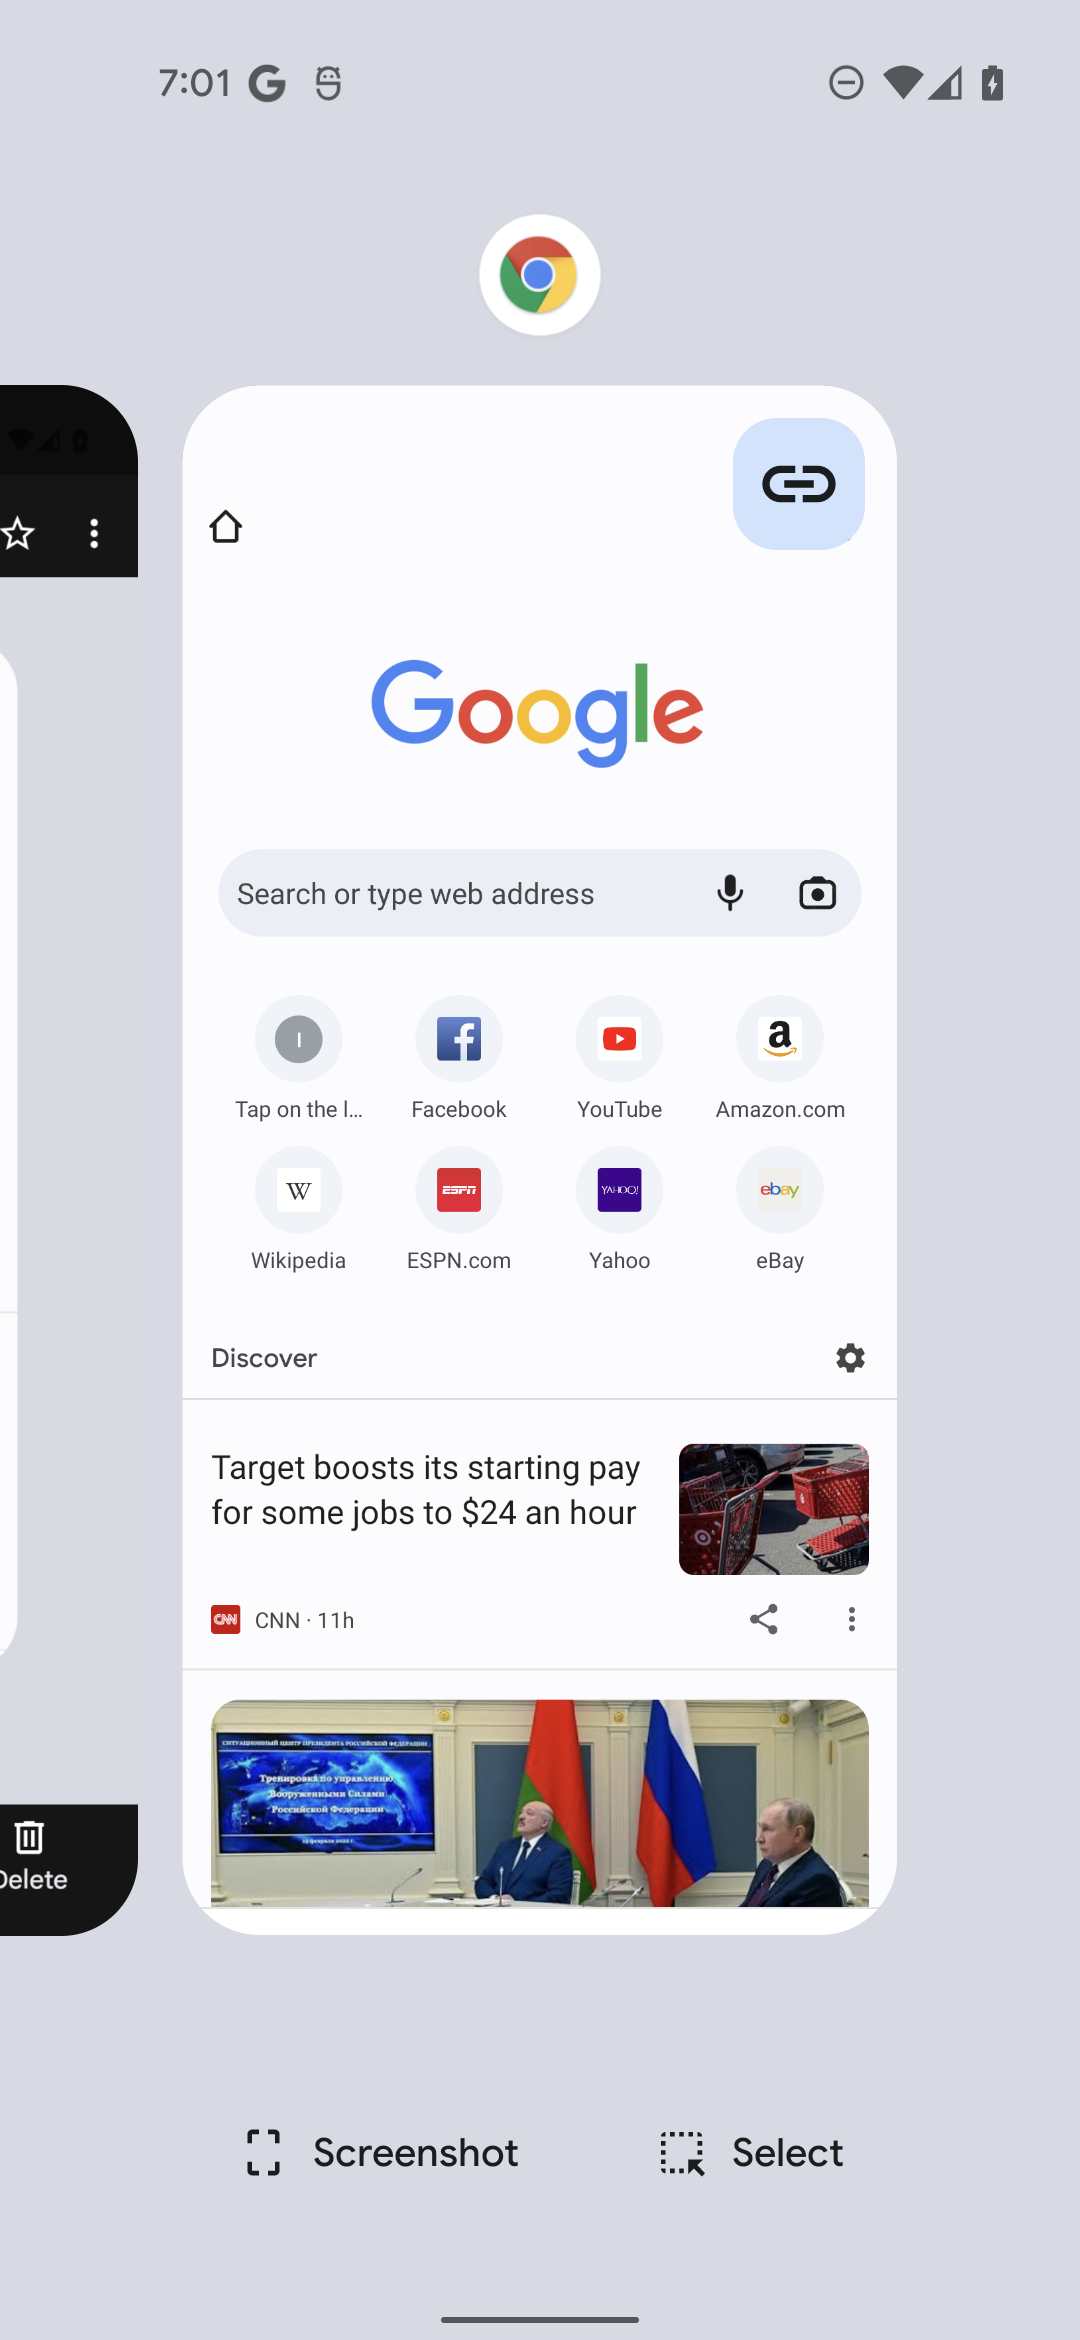
\includegraphics[width=0.8\columnwidth]{fig/recents-screen.pdf}
\caption{A screenshot of Recents screen showing that Chrome is recently accessed. However, a spyware app will not appear in the recent screen (if it chooses to hide from the recent screen), despite that one of its Activities is recently created and displayed.}
\label{fig:recents_screen}
\end{figure}


\subsubsection{Mitigations}
For apps that seek to hide their icons, our recommendation is that Android should enforce stricter requirements on what apps can hide icons (e.g., the three requirements from Android 10 build r1 to r14 mentioned in footnote~\ref{footnote:hide_icon}).
Most apps that run on Android phones should be required to have an icon. In the case of exploiting TV app features, while we
understand that running apps with only \texttt{LEANBACK\_LAUNCHER} activities on
Android phones increases compatibility, such a feature leads to abuse as Spy24
has already demonstrated.

Launching apps by predetermined signal from another app is not only used for
malicious purposes but also for benign purposes (e.g., dial pad can be used for
testing and numerous benign apps use a browser link to open themselves).
While browser links can be easily tracked by examining the manifest, currently
users have no way to discover if apps can launch themselves with hidden codes.
The difficulty is in part because hidden codes are used dynamically during
runtime: the outgoing dialed number is sent to apps, and apps can freely decide
what actions to perform based on the number received. This design makes it hard
for the Android system to identify what hidden numbers are being tracked by each
app.  One possible mitigation is to allow users to review apps that can receive predetermined signals (e.g., a list of apps that listen for the
\texttt{NEW\_OUTGOING\_CALL} intent or have intent filters for specific browser links,
perhaps as part of the privacy dashboard).

One potential fix to stop apps from hiding from the Recents screen is to enforce
having at least one activity per app in the Recents screen.




\subsection{Persistence}
\label{subsec:persistence}
This section describes the methods used by spyware apps to persist on the target
device by obscuring the uninstallation process and creating ``diehard'' services
(automatically restarting themselves after stops and reboots).

%\subsubsection{Capabilities}

\subsubsection*{Capability \#7: Obscuring the Uninstallation Process}

One way to prevent users from stopping and uninstalling an app is by
disabling the Force Stop and Uninstall buttons (see
Figure~\ref{fig:da} in the appendix).  For Android versions below 7.1,
these buttons can be disabled simply by registering the app with
\texttt{Device Administrator} (DA) privileges (as detailed in prior
work~\cite{shan2019device}). To enable these two buttons, the user
would have to deactivate the device administrator privileges for the
app.
%
Since Android 7.1, while the Force Stop button is disabled for DA
apps, the Uninstall button will remain enabled even if the app
registers as DA.  As a result, users can uninstall DA apps
directly~\cite{shan2019device}. Overall, we observe 11 apps that
register as DA.
%% \damon{this is really cryptic and difficult to
%% understand.}\alex{fixed}

Two apps, Cerberus and Mobile-tracker-free, directly interfere with the
uninstallation process, a behavior often observed in Android
malware~\cite{shan2019device,aljarrah2016maintaining}. Cerberus employs a series
of mechanisms to stop users from deactivating it as a DA app or
uninstalling it. These include trying to lock the device by invoking the
\texttt{lockNow} method of the \texttt{DevicePolicyManager} class and starting
an activity that blocks users from clicking on any buttons. Mobile-tracker-free,
on the other hand, tries to stop users from uninstalling it by starting an
Activity that blocks the uninstallation screen and requests a password set
by the abuser to proceed.

\subsubsection*{Capability \#8: Creating Diehard Services}
%\alex{a new title?}
%
Spyware apps strive to always be executing on the target device so
that they can collect as much information as possible.  We focus on
the ``diehard'' mechanisms that apps use to automatically restart
themselves after being stopped by the Android system (e.g., due to low memory) or after device
reboots. Echoing the diehard implementations discovered in prior
work~\cite{shao2019lightweight,zhou2020demystifying}, we observe two
main ways used by spyware apps to create diehard services. We also note
a third approach that appears to originate from the spyware ecosystem
and be a byproduct of other capabilities.

\textbf{Leveraging Scheduling Frameworks.} Scheduling frameworks such as
\texttt{JobScheduler}~\cite{JobSched94:online} and
\texttt{AlarmManager}~\cite{AlarmMan39:online} enable apps to repeatedly
restart. Apps can schedule to be restarted either when they are
first started or when they are being terminated by the system. To schedule
themselves to be restarted shortly after they are terminated, they override the
\texttt{onDestory} function, which is called before the app is terminated by the
system.

\textbf{Monitoring System Broadcasts.} Monitoring system broadcasts offers another way to wake up apps if they are not running already. Android sends broadcasts when various system events occur~\cite{Broadcas25:online}, and apps that monitor these system broadcasts will be woken up if they are not running already. Table~\ref{tab:monitor_broadcast} lists various systems broadcasts and the number of apps that monitor them.\footnote{Only a small number system broadcasts can be used to wake up apps after the restrictions introduced in Android 8~\cite{Implicit72:online}. We only consider these system broadcasts.} The spyware apps in our study predominantly use the \texttt{BOOT\_COMPLETED} broadcast. Monitoring
\texttt{BOOT\_COMPLETED} allows spyware apps to restart themselves
after the device reboots: the Android system will send a
\texttt{BOOT\_COMPLETED} system broadcast upon reboot, and spyware apps that listen
for this broadcast will automatically restart themselves. While \texttt{NEW\_OUTGOING\_CALL} and \texttt{SMS\_RECEIVED} are also popular, we note that they serve dual purposes (\texttt{NEW\_OUTGOING\_CALL} can be used to launch a hidden app and \texttt{SMS\_RECEIVED} can be used to monitor SMS messages).

\textbf{Listening for Accessibility or Notification Events.} Apps that register as an
\texttt{AccessibilityService} or
\texttt{NotificationListener- Service}
can also survive device
reboots. However, unlike the two techniques described above,
\texttt{AccessibilityService}
is less reliable because it can be
turned off by Android for battery saving reasons~\cite{AndroidA0:online,Accessib46:online}.


\begin{table}[t]
  \begin{tabular}{lr}
    System Broadcast         &\# of Apps  \\
    \midrule
    BOOT\_COMPLETED          &10          \\
    SMS\_RECEIVED            &9           \\
    NEW\_OUTGOING\_CALL      &9           \\
    PHONE\_STATE             &6           \\
    ACL\_DISCONNECTED        &1           \\
    ACL\_CONNECTED           &1           \\
    LOCKED\_BOOT\_COMPLETED  &1           \\
    WAP\_PUSH\_RECEIVED      &1           \\
  \end{tabular}
  \caption{System broadcasts and the number of apps monitoring them.\label{tab:monitor_broadcast}}
%  \vspace*{-1cm}
\end{table}


\begin{table*}[t]
	\centering
%	\begin{tabular}{l|m{2.5cm}|m{2.5cm}|m{3.2cm}|m{2.0cm}}
	\begin{tabular}{lm{1.8cm}m{2.0cm}m{3.1cm}m{2.6cm}m{2.6cm}}
%		\toprule
		Spyware Apps & Eavesdropping Sensitive PII & Cross-account Request Forgery & Unauthenticated Access to Victim Data & Poor Data Retention Practices & Unauthenticated SMS Commands \\
		\midrule
		mSPY & \partrating &  & Images &  &\\
		Mobile-tracker-free & & & Streaming & & \rating{100}\\
		Clevguard & \partrating & & Images* & &\\
\ltgrey 	HoverWatch & & & Audio* & &\\
\ltgrey 	Flexispy & \rating{100} & & Images/Audio* & &\\
\ltgrey		Spyic &  &  & Images* & \partrating &\\
		Spyhuman & & & Images/Audio & &\\
		TheTruthSpy & \rating{100} & \rating{100} & Images/Audio & \rating{100} &\\
		iKeyMonitor & & & & &\\
\ltgrey		Cerberus & & & Audio &  & \\
\ltgrey		Spy24 & & & Streaming* & &\\
\ltgrey		Spapp & & & Images/Audio/Streaming & \partrating & \rating{100}\\
		Meuspy & & & Images/Audio & \partrating &\\
		Highstermobile & & & Images &  &\\
%\ltgrey		LetMeSpy & & & & &\\
%		Spylive360 & & & Images/Audio & \rating{40} &\\
%		Talklog & & & & &\\
%		\bottomrule
	\end{tabular}
	\caption{Systematization of commodity spyware vulnerabilities. Circles denote the severity level of the insecurity. \protect \partrating\ indicates at least one instance of the insecurity; \protect \rating{100} indicates all app functionality is insecure; * indicates URLs are temporary and expire.
          Shading added to improve readability.
		%\sumanth{Should we move None's and No's to an empty circle? or leave that field blank? Also do we want to move the unauthenticated access column to circle's? If so we might lose information (e.g if just audio vs audio and images are affected. Suggestions?)} \geoff{(1) can you reorder the columns to match the order discussed in the section? (2) no column for SMS commands? (3) my preference is for blank cells over ``None''; (4) unauthenticated: as is conveys the info better than circles}
	}

	\label{tab:apps_spyware_vuln}
\end{table*}



%% \geoff{so ``waking
%% up apps'' is just for surviving reboots?  we might want to rename}\alex{fixed.
%% techinically apps can be woken up in many ways...after being stopped. by
%% \texttt{BOOT\_COMPLETED} seems to solely used for waking up purposes}

%We also note that the old \texttt{camera} framework has an API called
%\texttt{getSupportedPreviewSizes}, which supplies a list of supported preview
%sizes\alex{not sure about camera2 framework}.

%While the API document s

\subsubsection{Mitigations}
Apps that seek to persist by registering as device administrator will
no longer be successful as users can uninstall them on most devices
running Android 7.1 or above. For apps that seek to interfere with the
uninstallation process by creating activities or locking the device,
past literature on malware defense~\cite{fernandes2016android,
  aljarrah2016maintaining} has suggested improving attack detection
and introducing system level support for detecting and reacting when
an app window is covered.
% \geoff{are there suggestions from the malware papers?}\alex{fixed}


Prior work~\cite{zhou2020demystifying} has investigated various ways
of creating diehard apps. According to the authors, the diehard
mechanisms we observe are very resilient and can only be effectively
stopped via a force stop.
%% \geoff{``the above abuses can only be effectively stopped'' --- by abuse do you
%% mean spyware activities in general, or just the methods for keeping apps
%% alive/waking up apps?}\alex{fixed}
%% However, it is unlikely that users would force stop instead of
%% uninstall a suspicious app after they have discovered it.
Additionally, the fact that many spyware apps register as device administrator
creates another layer of complication --- while apps registered as DA may be
uninstalled directly after Android 7.1, the force stop option is disabled,
making it difficult for users to stop the spyware apps (unless they uninstall
it).
However, even if apps prevent a force stop, users can still uninstall
them.
We also recommend adding a dashboard for monitoring apps that will automatically
start themselves.\footnote{We note that some Android phones (e.g., Xiaomi) have a
built-in dashboard for managing apps that can automatically start
themselves~\cite{HowtoDis42:online}.}

%\geoff{so...no mitigation then?}\alex{fixed}


% \subsection{Discussion}
% TBD


% Before diving into the actual implementation, we first detail the general
% process of building customized camera implementations. Each camera is in
% Android is a \texttt{CameraDevice} and is responsible for producing raw data
% frames~\cite{Cameraca74:online}. Apps receive these raw data frames by
% specifying an output  buffer, which for example could be a
% \texttt{SurfaceView}, \texttt{ImageReader}, \texttt{RenderScript.Allocation},
% or \texttt{TextureView}~\cite{Cameraca74:online}.

% In practice, we observed X different customized camera implementations: (1)
% through creating 1x1 pixel SurfaceView.

% To create a camera session, provide it with one or more output target buffers
% your app can write output frames to.

% The first implementation creates 1x1 pixel previews. It requires the
% \texttt{SYSTEM\_ALERT\_WINDOW} permission to draw over other apps.
% Applications
